\documentclass[11pt,letterpaper]{article}

% ===================== PACKAGES =====================
\usepackage[utf8]{inputenc}
\usepackage[english]{babel}
\usepackage[T1]{fontenc}
\usepackage[margin=2.5cm]{geometry}
\usepackage{amsmath,amssymb}
\usepackage{graphicx}
\usepackage{booktabs}
\usepackage{array}
\usepackage{xcolor}
\usepackage{siunitx}
\usepackage{hyperref}
\usepackage{enumitem}
\usepackage{caption}
\usepackage{fancyhdr}
\usepackage{tcolorbox}
\usepackage{float}
\tcbuselibrary{skins,breakable}

\hypersetup{
    colorlinks=true,
    linkcolor=blue!50!black,
    citecolor=blue!50!black,
    urlcolor=blue!50!black
}

\sisetup{output-decimal-marker={.}, group-separator={,}}

\pagestyle{fancy}
\fancyhf{}
\fancyhead[L]{Adjustable Buck Converter (LM2596) -- Project Logbook}
\fancyhead[R]{\thepage}
\renewcommand{\headrulewidth}{0.4pt}

\newtcolorbox{pending}{colback=yellow!8,colframe=orange!60!black,arc=1mm,breakable,title={PENDING}}

% ===================== DOCUMENT METADATA =====================
\title{\textbf{Adjustable Step-Down Converter Based on the LM2596} \\[4pt]
\large Electronic Engineering Technical Documentation}
\author{Project Logbook}
\date{Version 0.1 --- \today}

\begin{document}

\maketitle

\begin{abstract}
\noindent This document describes the design, KiCad schematic/PCB layout, and COMSOL thermal validation of
an adjustable step-down (buck) power supply built around the LM2596S-ADJ switching regulator. It follows
the same project series as the LM317 linear adjustable supply (\texttt{FuenteLM317\_9V}): a quick,
practical exercise meant primarily to build real PCB layout experience (placement, routing priorities, a
ground-plane strategy, via stitching under a thermal pad) and to validate the result thermally, before
moving on to multiphase VRM work. Documented as an honest engineering logbook: every result is marked as
\textbf{calculated}, \textbf{simulated}, or \textbf{pending} -- never filled in with invented placeholder
data. LTspice simulation of the closed loop was deliberately skipped for this project (see
Section~\ref{sec:design}): the topology and component values are taken directly from the manufacturer's
own validated application circuit, so re-deriving them in SPICE would have added time without adding
information. \textbf{Key result}: at the demonstration operating point (\SI{12}{\volt}
$\to$ \SI{2}{\volt}, \SI{0.5}{\ampere}), COMSOL gives \SI{0.444}{\watt} total estimated loss, with the
LM2596's junction at \SI{44.3}{\celsius} and the catch diode (the hottest point on the board) at
\SI{52.5}{\celsius} -- both comfortably under their rated limits. A separate worst-case sweep
(\SI{35}{\volt}$\to$\SI{1.23}{\volt}, the extreme low-duty-cycle end of the adjustable range) found that
the catch diode, not the regulator IC, is the component that actually limits the safe operating envelope,
exceeding its rated junction temperature above $\approx$\SI{1.5}{}--\SI{2}{\ampere} in the conservative
(no-radiation) case. This is documented as a known limitation with a proposed, not-yet-implemented fix.
\end{abstract}

\tableofcontents
\newpage

% ======================================================================
\section{Project Objective}

Design, lay out, and thermally validate an adjustable step-down converter using a real integrated buck
regulator (LM2596S-ADJ), with two explicit goals: (1) build hands-on KiCad PCB layout experience --
component placement for a switching converter, trace-width sizing, a two-layer ground-plane strategy, and
via stitching under a thermal pad -- as a deliberately fast, low-complexity exercise before the next
multiphase VRM project; and (2) validate the design thermally in COMSOL, in the same style as the LM317
project, so the two can be compared directly (Section~\ref{sec:conclusions}).

% ======================================================================
\section{Reference Design}
\label{sec:design}

\subsection{Why no closed-loop SPICE simulation}

Unlike the LM317 and VRM projects in this series, this project does \textbf{not} include an LTspice
closed-loop simulation of the LM2596. The topology and component values below are taken directly from the
manufacturer's own datasheet application circuit (Texas Instruments LM2596 datasheet, Figure 30: ``1.2 to
35\,V Adjustable 3.0\,A Power Supply with Low Output Ripple''), which is itself a validated, published
reference design. Re-deriving a SPICE model for an extremely standard, widely-used topology would have
repeated work the manufacturer already did, without adding new information -- so the LTspice step was
intentionally skipped to prioritize time on the PCB layout and the thermal validation, which \emph{are}
specific to this board.

\subsection{Topology and component values (adopted from the datasheet)}

\begin{center}
\begin{tabular}{@{}ll@{}}
\toprule
U1 & LM2596S-ADJ (adjustable step-down regulator, TO-263-5 / PowerPAK-style SMD package) \\
C1 (input) & \SI{100}{\micro\farad}, rated $\geq$\SI{50}{\volt} (covers the \SI{40}{\volt} max input) \\
D1 (catch diode) & SS34 Schottky, \SI{3}{\ampere}/\SI{40}{\volt} (SMD substitute for the datasheet's 1N5822, same ratings) \\
L1 & \SI{33}{\micro\henry} \\
C2 (output) & \SI{220}{\micro\farad} \\
RV1 & \SI{50}{\kilo\ohm} trimmer potentiometer (feedback, adjustable) \\
R1 & \SI{1.21}{\kilo\ohm} (feedback, fixed) \\
L2, C3 (optional output ripple filter) & \SI{20}{\micro\henry}, \SI{100}{\micro\farad} \\
\bottomrule
\end{tabular}
\end{center}

Output voltage range (datasheet formula, $V_{ref}\approx\SI{1.23}{\volt}$):
\begin{equation}
V_{out} = V_{ref}\left(1+\frac{R_{RV1}}{R_1}\right)
\end{equation}
With $R_1=\SI{1.21}{\kilo\ohm}$ and $RV1$ swept 0 to \SI{50}{\kilo\ohm}: $V_{out}$ spans
\SI{1.23}{\volt} (RV1 at \SI{0}{\ohm}) up to the catalog figure's stated \SI{35}{\volt} at a
partial (not full-scale) RV1 setting -- the datasheet's own ``1.2 to 35\,V'' range does not correspond to
the pot's full \SI{0}{}--\SI{50}{\kilo\ohm} travel at these exact R1/RV1 values (full travel would
mathematically reach $\approx$\SI{52}{\volt}), so the usable \SI{35}{\volt} ceiling is set by the
pot position, not derived from scratch here -- adopted as given in the reference.

The optional output ripple filter (L2/C3) sits \emph{after} the point where feedback is sensed -- the
regulator regulates the pre-filter node, and L2/C3 only clean up additional high-frequency ripple on top
of that already-regulated voltage, so the extra filter does not fight the control loop.

% ======================================================================
\section{KiCad Schematic and PCB}
\label{sec:pcb}

\subsection{Footprint selection}

\begin{center}
\resizebox{\textwidth}{!}{%
\begin{tabular}{@{}lll@{}}
\toprule
Part & Footprint & Note \\
\midrule
U1 (LM2596S-ADJ) & \texttt{Package\_TO\_SOT\_SMD:TO-263-5\_TabPin3} & Stock KiCad symbol/footprint pair \\
D1 (SS34) & \texttt{Diode\_SMD:D\_SMC} & SMD, same 3A/40V rating as the datasheet's 1N5822 \\
C1, C2, C3 & \texttt{Capacitor\_THT:CP\_Radial\_D8.0mm\_P3.50mm} / \texttt{D10.0mm\_P5.00mm} & Sized per value/voltage, Section~\ref{sec:caps} \\
RV1 (50k trimmer) & \texttt{Potentiometer\_THT:Potentiometer\_Bourns\_3266Y\_Vertical} & Real, common part \\
R1 & \texttt{Resistor\_SMD:R\_0805\_2012Metric} & Consistency with the rest of the SMD parts \\
L1, L2 & \texttt{Inductor\_SMD:L\_12x12mm\_H4.5mm} & SMD shielded power inductor (no 3D model in the KiCad library, see Section~\ref{sec:thermal-model}) \\
TP1--TP4 (I/O) & \texttt{TestPoint:TestPoint\_THTPad\_3.0x3.0mm\_Drill1.5mm} & Bare solder pads, not a connector housing \\
\bottomrule
\end{tabular}}
\end{center}

\subsection{Capacitor sizing}
\label{sec:caps}

Radial electrolytic package sizes were chosen from the actual voltage rating each capacitor needs, not a
single generic size for all three:

\begin{center}
\begin{tabular}{@{}llll@{}}
\toprule
Cap & Value & Voltage needed & Typical minimum can size \\
\midrule
C1 & \SI{100}{\micro\farad} & $\sim$\SI{50}{\volt} & $\varnothing$\SI{8}{}x\SI{11.5}{\milli\meter} \\
C2 & \SI{220}{\micro\farad} & $\sim$\SI{35}{\volt} & $\varnothing$\SI{10}{}x\SI{12.5}{\milli\meter} \\
C3 & \SI{100}{\micro\farad} & $\sim$\SI{35}{\volt} & $\varnothing$\SI{8}{}x\SI{11.5}{\milli\meter} \\
\bottomrule
\end{tabular}
\end{center}

\begin{pending}
These are typical catalog sizes for the stated value/voltage, not a specific vendor part number verified
against a real datasheet (unlike the LM317 project's heatsink and capacitor choices). Low risk for a
layout-practice board, but should be confirmed if this were ever built.
\end{pending}

\subsection{Layout priorities applied}

Following the TI application note's own layout guidance (``locate the programming resistors near the
feedback pin using short leads'' and ``keep feedback wiring away from inductor flux''):

\begin{itemize}[nosep]
    \item RV1/R1 (the feedback divider) placed with short, direct traces to the FB pin, and physically
    separated from L1's body -- not adjacent to it the way some low-cost commercial LM2596 modules do
    (a deliberate choice discussed and compared against a real commercial module photo during layout).
    \item High-current power traces (V\_in, the switch node, L1--C2--L2--C3, V\_out) sized to
    $\approx$\SI{1.3}{\milli\meter} (conservative, 10\textdegree C-rise IPC-2221 estimate for
    \SI{3}{\ampere} on \SI{1}{oz} copper) -- not ``as narrow as possible'', which was an incorrect
    instinct corrected during layout. Control/feedback traces (FB, ON/OFF) kept narrow, since they carry
    negligible current and narrower traces reduce coupling area.
    \item Short, direct traces between U1's output, D1, and L1 (the switching loop) instead of a copper
    pour -- at \SI{3}{\ampere} and with a simple linear (non-branching) node topology, a pour was judged
    unnecessary (see Section~\ref{sec:conclusions} discussion, contrasted with the VRM project's switch
    node, where a pour was the right call at \SI{10}{}--\SI{20}{\ampere}).
\end{itemize}

\subsection{Ground strategy}

Two-layer board (unlike the VRM project's four layers -- a single ground domain and \SI{3}{\ampere} do
not justify the extra layers and SGND/PGND split that the VRM required). Top layer: components and all
signal/power routing. Bottom layer: a solid ground pour, connected up via stitching vias placed next to
each ground pad (not via-in-pad, to avoid a solder-wicking risk relevant on a board meant to represent
real assembly practice) -- through-hole parts' own leads double as their via where the lead already
reaches the bottom layer.

\subsection{Via stitching under U1's thermal pad}

U1's exposed GND/thermal pad (pin 3 of the TO-263-5) is stitched to the bottom-layer ground plane with
\textbf{9 vias} in an even $3\times3$ grid, standard via size, well clear of the pad edge. This is more
than the $4$--$6$ vias that would be strictly necessary at \SI{3}{\ampere} for this package, but causes no
harm; it was kept rather than reworked.

\subsection{ERC / DRC}

Schematic ERC and PCB DRC both clean (confirmed in KiCad, no outstanding violations). Not intended for
fabrication.

% ======================================================================
\section{Thermal Simulation (COMSOL)}
\label{sec:thermal}

\subsection{Methodology}

\textit{Heat Transfer in Solids}, natural convection, \SI{25}{\celsius} quiescent ambient air, no
heatsink. The PCB copper (top/bottom masks) and component geometry were exported from the KiCad design
(\texttt{fem/geometria/LM259.step}, \texttt{Arreglo.step}, plus the copper mask text files) and imported
into COMSOL. Heat sources (U1, D1, L1, L2) are driven by \textbf{analytically estimated losses}, not
measured or chip-vendor-simulated values:

\begin{pending}
The loss values feeding every thermal result below are datasheet-derived estimates ($V_{sat}$ and $V_f$
taken at their \SI{3}{\ampere} values and held \emph{constant} at every current -- conservative at lower
currents, where the real drops are smaller -- plus an assumed \SI{100}{\nano\second} switching
transition time; exact formulas in Section~\ref{sec:thermal-model}) -- not measured hardware data, and not output from a manufacturer SPICE model (none is
available for the LM2596; see the project's earlier LTspice-vs-COMSOL tooling discussion). The COMSOL
\emph{thermal} solve itself is a genuine FEM result for whatever loss number it is given; the uncertainty
is entirely in that input loss estimate, which is conservative by construction (ignores radiative cooling,
discussed next).
\end{pending}

\subsection{Model setup in detail}
\label{sec:thermal-model}

\paragraph{Software and workflow.} COMSOL Multiphysics 6.4, driven entirely from Python (\texttt{MPh}
library) so every model can be rebuilt from scratch: scripts in \nolinkurl{fem/codigo/}. The final model file
is \nolinkurl{fem/BUCK_LM2596_termico_STEP.mph} (worst-case sweep and variants) and
\nolinkurl{fem/BUCK_LM2596_termico_12V_2V_05A.mph} (demonstration point). The hand-prepared geometry
file \nolinkurl{fem/BUCK_LM2596_termico.mph} is never modified by the scripts; everything is written to new
files.

\paragraph{Geometry.} The board was exported from KiCad as STEP and imported into COMSOL by hand
(\textit{Form Union}, so touching parts share faces and no manual contact pairs are needed -- unlike the
LM317 project). From that import the scripts then:
\begin{itemize}[nosep]
    \item \textbf{remove} the STEP's copper solids (48 track/zone objects, 106 pads, 32 via barrels/cores,
    and the separate \SI{35}{\micro\meter} B.Cu plane object), which could not be meshed within the
    available memory (Section~\ref{sec:debug-log}); copper is modeled as a thin layer instead (below);
    \item \textbf{add solder blocks} (SAC305) under U1's tab, under D1's two terminals and under U1's five
    pin feet: KiCad's 3D models start at $z=\SI{1.595}{\milli\meter}$ while the board top is at
    \SI{1.51}{\milli\meter}, so without them the components float $\approx$\SI{85}{\micro\meter} above
    the board and are thermally disconnected (the LM317 ``disconnected assembly'' problem in a new form);
    \item \textbf{add 16 vias} as solid cylinders ($\varnothing$\SI{0.3}{\milli\meter}) at the exact KiCad
    via positions, with an equivalent conductivity $k_{via}=\SI{122}{\watt\per\meter\per\kelvin}$
    (\SI{25}{\micro\meter} copper barrel in a \SI{0.3}{\milli\meter} drill);
    \item \textbf{add L1/L2 pads} as \SI{40}{\micro\meter} copper blocks. The inductor \emph{bodies} are
    not modeled: KiCad has no 3D model for \texttt{L\_12x12mm\_H4.5mm}, they are not in the main heat
    path, and their losses enter through their pads (conservative: the bodies' extra cooling area is
    missing). RV1 is also omitted (negligible current, no dissipation).
\end{itemize}

\paragraph{Copper as a thin layer with the real layout.} The F.Cu and B.Cu layers were exported from KiCad
as SVG (\texttt{kicad-cli pcb export svg}, board area only), rasterized at \SI{0.1}{\milli\meter} and
stored as copper-fraction maps (\nolinkurl{fem/geometria/mascara_cobre_F.txt}, \texttt{\_B.txt}; F.Cu
\SI{19.5}{\percent} coverage = pads and tracks, B.Cu \SI{93.3}{\percent} = ground pour). Each map drives a
COMSOL \textit{Thin Layer} (conductive, \SI{35}{\micro\meter}) on the board's top/bottom face with
$k = k_{FR4} + (k_{Cu}-k_{FR4})\cdot m(x,y)$, so every track, pad and pour clearance conducts exactly where
it is on the real board, without meshing \SI{35}{\micro\meter} solids. Note: the F.Cu ground zone exists
in the KiCad file but is \emph{unfilled}, so it is (correctly) not in the map.

\paragraph{Materials.}
\begin{center}
\small
\begin{tabular}{@{}lccc l@{}}
\toprule
Part & $k$ [\si{\watt\per\meter\per\kelvin}] & $\rho$ [\si{\kilogram\per\cubic\meter}] & $C_p$ [\si{\joule\per\kilogram\per\kelvin}] & Source \\
\midrule
FR4 board & 0.3 & 1900 & 1369 & typical \\
Copper (tab, pins, layers, L pads) & 400 & 8960 & 385 & standard \\
Vias (equivalent) & 122 (0.3 off) & 8960 & 385 & barrel geometry \\
Solder SAC305 & 58 & 7400 & 230 & typical \\
EMC (U1 and D1 bodies) & 0.7 & 1900 & 900 & as LM317 \\
Filler (C1--C3, R1) & 0.2 & 1050 & 1400 & as LM317 \\
\bottomrule
\end{tabular}
\end{center}
Only $k$ matters for the stationary results reported here.

\paragraph{Heat sources (all in \textit{Heat rate} mode, i.e. total watts).}
U1 on the internal face between its copper tab and the plastic body (where the die sits, as in the LM317
model); D1 on the faces where its terminals meet the solder; L1/L2 on the top faces of their pads. Losses
($V_{sat}=\SI{1.16}{\volt}$, $I_q=\SI{5}{\milli\ampere}$, $f_{sw}=\SI{150}{\kilo\hertz}$ from the TI
datasheet; $V_f=\SI{0.5}{\volt}$ from the SS34 datasheet maximum; $t_{sw}=\SI{100}{\nano\second}$,
$DCR_1=\SI{40}{\milli\ohm}$, $DCR_2=\SI{25}{\milli\ohm}$ \textbf{assumed}):
\begin{gather*}
D=\frac{V_{out}+V_f}{V_{in}-V_{sat}+V_f},\qquad
P_{U1}=V_{sat}I_{out}D+\tfrac12 V_{in}I_{out}t_{sw}f_{sw}+V_{in}I_q,\\
P_{D1}=V_f I_{out}(1-D),\qquad P_{L1}=I_{out}^2 DCR_1,\qquad P_{L2}=I_{out}^2 DCR_2 .
\end{gather*}

\paragraph{Convection.} Same criterion as the LM317 project (one correlation per face orientation, no air
domain), but written as explicit expressions because COMSOL's built-in natural-convection correlations
returned NaN in this model (Section~\ref{sec:debug-log}). A single \textit{Heat Flux} on every exterior
face picks the correlation from the face normal: horizontal plate facing up
($Nu=0.54\,Ra^{1/4}$, or $0.15\,Ra^{1/3}$ above $10^7$) and facing down ($Nu=0.27\,Ra^{1/4}$) with
$L=\SI{10}{\milli\meter}$ (board area/perimeter), vertical wall (Churchill--Chu) with
$L=\SI{5}{\milli\meter}$; air properties at the film temperature. Radiation (surface-to-ambient,
$\varepsilon=0.9$) is available as a switch and \emph{off} in all design-relevant results.

\paragraph{Mesh and studies.} Free tetrahedra with the geometry stretched $10\times$ in $z$ while meshing
(\texttt{zscale}), so thin parts get flat elements instead of millions of tiny ones: 110,446 elements.
Studies: (1) single operating point, (2) $I_{out}$ sweep \SIrange{0.5}{3}{\ampere}, (3) variants
(vias on/off, radiation on/off, L losses on/off). Solved with a \SI{8}{\giga\byte} memory cap
(\texttt{systemd-run -p MemoryMax}) after an earlier unbounded run crashed the machine.

\subsection{Demonstration operating point: \SI{12}{\volt}$\to$\SI{2}{\volt} at \SI{0.5}{\ampere}}

This is the same load condition used for the LM317 comparison in the companion project, so the two can be
compared on equal footing.

\begin{center}
\begin{tabular}{@{}ll@{}}
\toprule
Duty cycle (real, incl. $V_f$/$V_{sat}$ drops) & $0.2205$ \\
$P_{U1}$ & \SI{0.2329}{\watt} \\
$P_{D1}$ & \SI{0.1949}{\watt} \\
$P_{L1}$ & \SI{0.010}{\watt} \\
$P_{L2}$ & \SI{0.00625}{\watt} \\
$P_{tot}$ & \SI{0.444}{\watt} \\
Output power & \SI{1.0}{\watt} \\
Estimated efficiency & \SI{69.25}{\percent} \\
U1 junction (tab-body face) & \SI{44.29}{\celsius} \\
D1 max (hottest point on the board) & \SI{52.49}{\celsius} \\
\bottomrule
\end{tabular}
\end{center}

\begin{figure}[H]
\centering
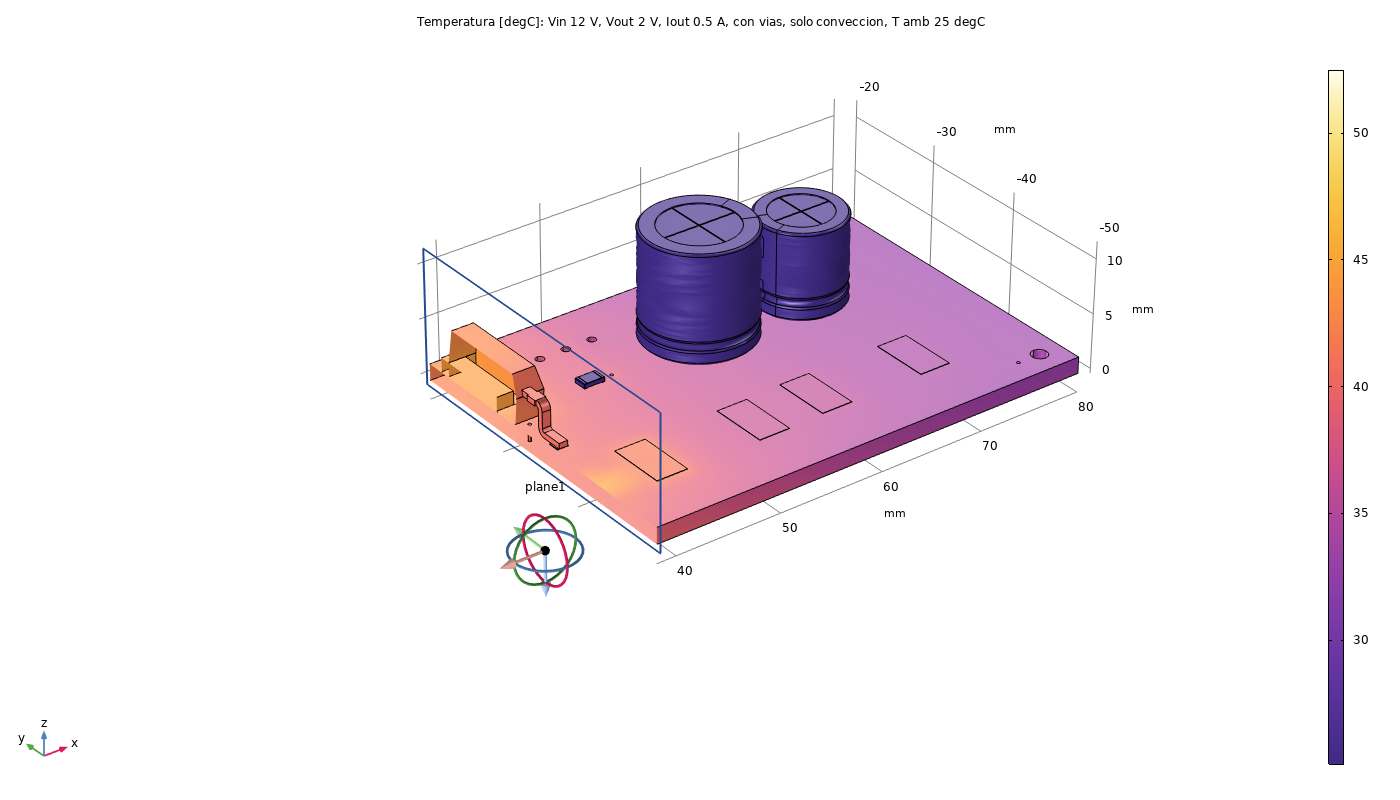
\includegraphics[width=0.75\textwidth]{../fem/figuras/temperatura_3D_12V_2V_05A.png}
\caption{Temperature map, demonstration point (\SI{12}{\volt}$\to$\SI{2}{\volt}, \SI{0.5}{\ampere}, with
vias, convection only). Scale \SI{25}{}--\SI{55}{\celsius}.}
\label{fig:t-demo}
\end{figure}

Both results sit well under their rated limits (\SI{125}{\celsius}). Note the estimated efficiency here
(\SI{69}{\percent}) is \emph{not} representative of a buck converter's typical best-case figure
(\SI{85}{}--\SI{95}{\percent}, quoted as general knowledge, not as a claim about this specific operating
point) -- a \SI{2}{\volt} output next to a Schottky diode's $\approx$\SI{0.5}{\volt} forward drop is an
inherently unfavorable ratio for a non-synchronous topology; see the worst-case sweep below for where this
effect is most pronounced.

\subsection{Worst-case sweep: \SI{35}{\volt}$\to$\SI{1.23}{\volt} (minimum duty cycle)}

A second analysis deliberately targets the adjustable range's extreme low-duty-cycle end -- maximum input
voltage, minimum output voltage -- where the catch diode conducts for the largest fraction of the
switching period (duty cycle $D=(V_{out}+V_f)/(V_{in}-V_{sat}+V_f)\approx\SI{5.0}{\percent}$ including
the diode and switch drops, so D1 conducts $\approx$\SI{95}{\percent} of the time).

\begin{center}
\begin{tabular}{@{}cccc@{}}
\toprule
$I_{out}$ & $P_{tot}$ & U1 junction & D1 max \\
\midrule
\SI{0.5}{\ampere} & \SI{0.59}{\watt} & \SI{50.4}{\celsius} & \SI{58.9}{\celsius} \\
\SI{1.0}{\ampere} & \SI{1.04}{\watt} & \SI{63.8}{\celsius} & \SI{85.4}{\celsius} \\
\SI{1.5}{\ampere} & \SI{1.52}{\watt} & \SI{77.0}{\celsius} & \SI{111.4}{\celsius} \\
\SI{2.0}{\ampere} & \SI{2.03}{\watt} & \SI{90.0}{\celsius} & \SI{136.9}{\celsius} \\
\SI{2.5}{\ampere} & \SI{2.57}{\watt} & \SI{103.1}{\celsius} & \SI{162.5}{\celsius} \\
\SI{3.0}{\ampere} & \SI{3.15}{\watt} & \SI{116.2}{\celsius} & \SI{187.9}{\celsius} \\
\bottomrule
\end{tabular}
\end{center}

\begin{figure}[H]
\centering
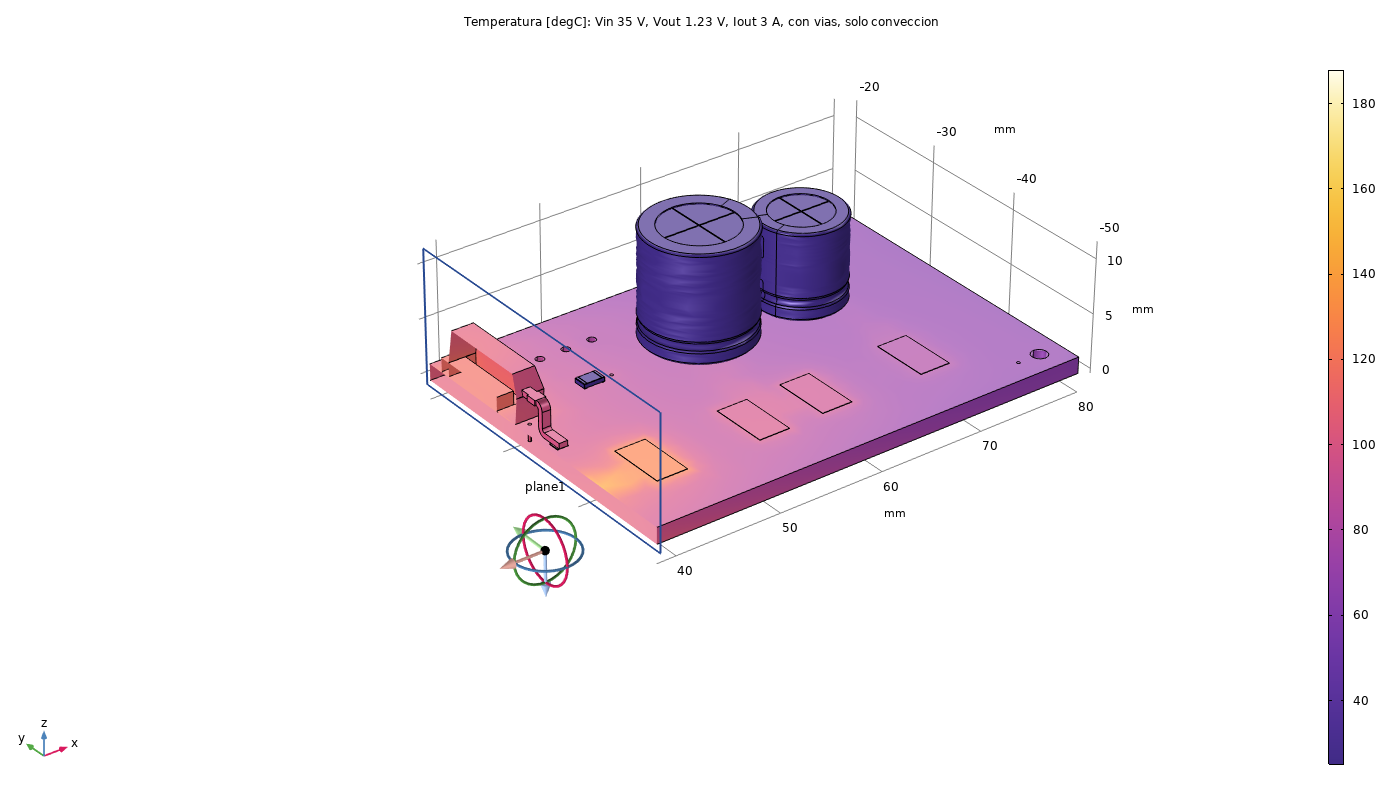
\includegraphics[width=0.75\textwidth]{../fem/figuras/temperatura_3D_nominal.png}
\caption{Temperature map, worst case at \SI{3}{\ampere} (\SI{35}{\volt}$\to$\SI{1.23}{\volt}, with vias,
convection only). Scale \SI{25}{}--\SI{190}{\celsius}; the hot spot is D1's anode terminal
(Section~\ref{sec:d1-fix}).}
\label{fig:t-worst}
\end{figure}

\textbf{Key finding: the catch diode D1, not the LM2596 itself, is the component that limits the safe
operating envelope.} The SS34's rated junction temperature is \SI{125}{}--\SI{150}{\celsius} depending on
the manufacturer; in this conservative (no-radiation) case, D1 exceeds that limit somewhere between
\SI{1.5}{} and \SI{2}{\ampere} at this voltage extreme, while U1 itself stays under \SI{125}{\celsius}
through the full \SI{3}{\ampere} sweep (with little margin left at the top end).

\subsubsection{Variants at \SI{3}{\ampere} (worst case)}

\begin{center}
\begin{tabular}{@{}lcc@{}}
\toprule
Variant & U1 junction & D1 max \\
\midrule
With vias (base case) & \SI{116.2}{\celsius} & \SI{187.9}{\celsius} \\
Without vias & \SI{123.8}{\celsius} (+8) & \SI{205.2}{\celsius} (+17) \\
With vias + radiation ($\varepsilon=0.9$) & \SI{89.3}{\celsius} & \SI{155.8}{\celsius} \\
Without vias + radiation & \SI{96.7}{\celsius} & \SI{170.6}{\celsius} \\
With vias, no L1/L2 losses & \SI{108.5}{\celsius} & \SI{180.6}{\celsius} \\
\bottomrule
\end{tabular}
\end{center}

\begin{figure}[H]
\centering
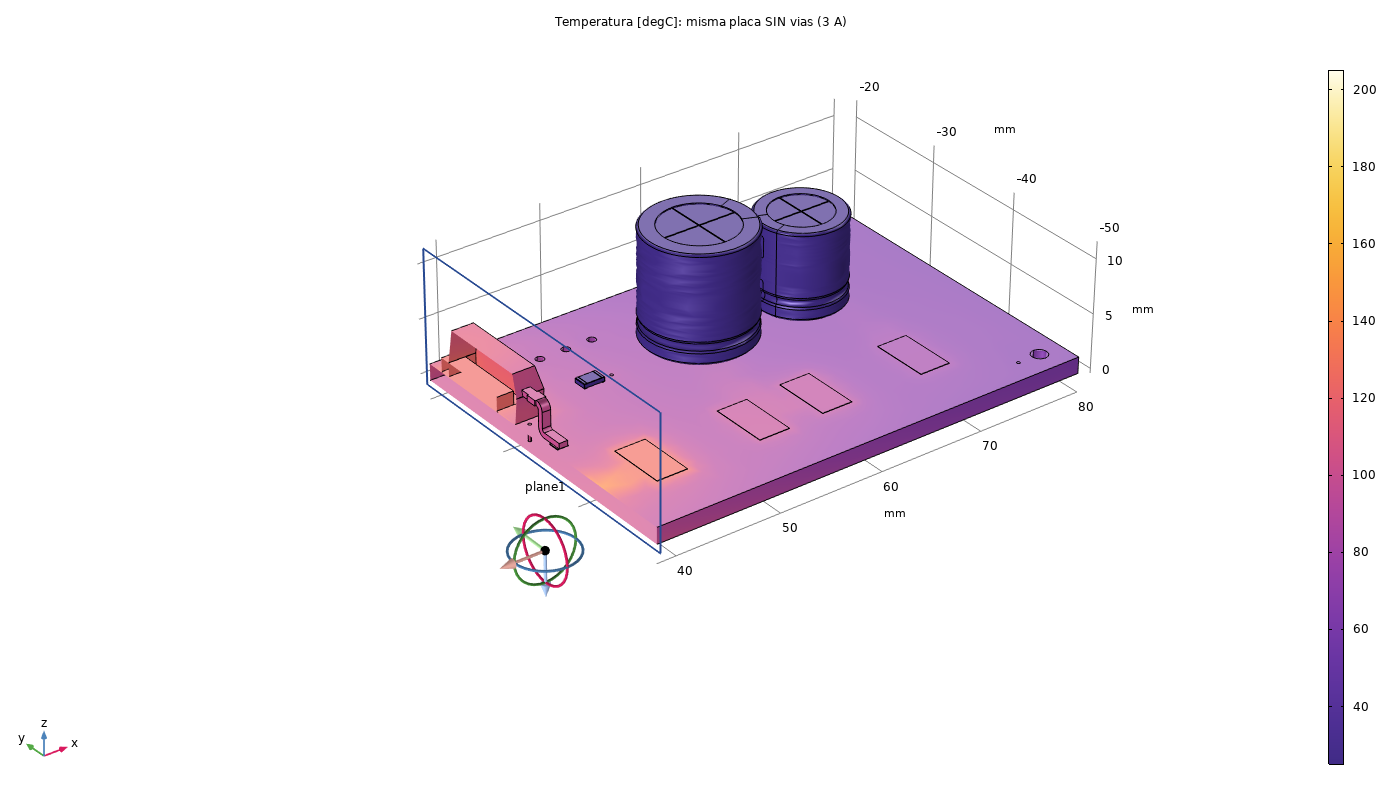
\includegraphics[width=0.75\textwidth]{../fem/figuras/temperatura_3D_sin_vias.png}
\caption{Same worst-case condition, \textbf{without} via stitching under U1's thermal pad. Scale
\SI{25}{}--\SI{205}{\celsius}. Compare against Figure~\ref{fig:t-worst} (with vias) -- the hot spot stays
at D1's anode either way, confirming the vias help U1 and D1 globally but do not address D1's locally
isolated terminal (Section~\ref{sec:d1-fix}).}
\label{fig:t-novias}
\end{figure}

Via stitching under U1's thermal pad does help (\SI{8}{\celsius} on U1, \SI{17}{\celsius} on D1 at the
worst point), but is not sufficient on its own to bring D1 under its limit at high current. Radiative
cooling is large (\SI{27}{}--\SI{32}{\celsius}) but was not used as design margin, since it is not
guaranteed in an enclosure -- the convection-only case is treated as the design-relevant one throughout.

\subsection{Root cause and proposed improvement}
\label{sec:d1-fix}

The \SI{187.9}{\celsius} peak on D1 is localized at its anode terminal -- the point where the heat
source enters the model. That terminal lands on a ground pad that is isolated from the main ground pour,
connected to GND by only a single via. The board's center-of-die temperature a few millimeters away is
much lower ($\approx$\SI{122}{\celsius} under D1's body center at the same worst-case point), consistent
with that terminal specifically being under-connected thermally, not the whole diode footprint.

\begin{pending}
\textbf{Proposed improvement, not implemented in this revision:} extend the F.Cu ground pour around D1's
anode pad and add more stitching vias there, matching what was already done for U1's thermal pad. Expected
to meaningfully reduce the \SI{187.9}{\celsius} figure, based on the \SI{17}{\celsius} improvement vias
already produced elsewhere on the same net -- not re-simulated to confirm the exact new number, since
reworking the layout for this one finding was judged not worth it for a layout-practice project at this
stage (see discussion in Section~\ref{sec:conclusions}).
\end{pending}

\subsection{Modeling and debugging log}
\label{sec:debug-log}

In order, every problem found while building the model and what was done about it. Several early numbers
were wrong and are recorded here explicitly so they are never reused.

\begin{enumerate}[nosep]
    \item \textbf{First model built from primitives} (blocks/cylinders with dimensions read from the KiCad
    STEP via FreeCAD). Superseded once the full STEP import was done by hand in COMSOL, which is the
    geometry used for all results.
    \item \textbf{Built-in natural convection returned NaN.} Isolated by switching boundary features on one
    at a time on a model that solved with a fixed temperature: the \textit{Horizontal plate, upside}
    correlation (and, once replaced, the downside one) produced NaN even with a raised initial
    temperature or different characteristic lengths. Fix: the same correlations written explicitly
    (Section~\ref{sec:thermal-model}), with a floor on $\Delta T$ and an initial temperature
    \SI{20}{\kelvin} above ambient (the $\Delta T^{1/4}$ term has an infinite derivative at
    $\Delta T=0$).
    \item \textbf{Empty heat-source selection.} A box selection meant to catch U1's tab/body face caught
    nothing (``inside'' condition with a face edge exactly on the box limit), so \SI{1.1}{\watt} was spread
    over zero area. Fix: ``intersects'' selections in the middle of each part, and every source selection
    is now checked to be non-empty before solving. A second version caught too many faces (side walls of
    solder and pads); fixed with one ``inside'' box per terminal/pad.
    \item \textbf{Solder gap.} Discovered by measuring every one of the 271 imported domains: components
    start at $z=\SI{1.595}{\milli\meter}$ and copper ends at \SI{1.55}{\milli\meter}. Fixed with the
    solder blocks above.
    \item \textbf{STEP copper could not be meshed.} With the imported \SI{35}{}--\SI{40}{\micro\meter}
    copper laminae and \SI{25}{\micro\meter} via barrels, the mesher failed with ``intersecting edge
    elements'' at a different tiny feature each time (test-point pads, via annular rings), for four
    different size/scaling combinations. A finer mesh used \SI{11.5}{\giga\byte} of RAM and was killed by
    the operating system (out of memory), taking the desktop session with it. Fix: copper as a thin
    layer with the real layout (Section~\ref{sec:thermal-model}), which meshes in seconds.
    \item \textbf{Copper map unit bug -- first results invalid.} The interpolation function ignored its
    ``mm'' argument unit and read coordinates in metres, so the copper map evaluated to 0 everywhere and
    the board behaved as bare FR4. Detected because the bottom ground plane ranged
    \SIrange{25}{253}{\celsius} (a solid copper plane must be nearly isothermal). The results from that
    run (U1 \SI{154.6}{\celsius}, D1 \SI{319.6}{\celsius} at \SI{35}{\volt}/\SI{3}{\ampere}) are
    \textbf{invalid}. Fix: dimensionless arguments in mm; verified that the map is 1 in the middle of the
    ground plane and that the plane is now nearly isothermal. All numbers in this report come from the
    corrected model.
    \item \textbf{Sweep results read incorrectly}, then fixed: a sweep of a non-geometric parameter is
    stored by COMSOL as inner solutions of one dataset, not as outer ones.
\end{enumerate}

\subsection{Refinements attempted but not adopted}
\label{sec:attempts}

Two refinements were attempted for the demonstration point (\SI{12}{\volt}$\to$\SI{2}{\volt},
\SI{0.5}{\ampere}) to cross-check the adopted model. \textbf{Neither produced a valid result}; they are
documented so the attempt is not repeated blindly.

\paragraph{Solid copper from the STEP} (\nolinkurl{fem/BUCK_LM2596_termico_STEP_cobre.mph}). Same model,
but keeping the STEP's tracks, pads and ground plane as solids. An automatic loop refined the mesh only
around each location where the mesher failed (\nolinkurl{fem/codigo/malla_automatica.py}). After nine local
refinements, each new attempt taking longer (\SI{1}{}$\to$\SI{17}{\minute}), the job exceeded a
\SI{14}{\giga\byte} memory cap and was killed. \textbf{Conclusion:} not feasible on this machine (23 GB
RAM); the thin-layer model, which uses the same real copper layout, is the adopted one.

\paragraph{Conjugate heat transfer with simulated air} (\nolinkurl{fem/BUCK_LM2596_termico_12V_2V_05A_aire.mph}).
Instead of convection correlations, an air box around the board (finally
\SI{100}{}$\times$\SI{70}{}$\times$\SI{75}{\milli\meter}, open boundaries at \SI{25}{\celsius}) with
laminar flow, gravity and the \textit{Non-Isothermal Flow} coupling (air as an ideal gas, so its density
change drives the buoyancy). Copper as thin layer; THT holes filled with solder and capacitor leads cut
at the board surface (both needed for the air to mesh). Attempts:
\begin{center}
\small
\begin{tabular}{@{}p{6.3cm}p{8.2cm}@{}}
\toprule
Attempt & Outcome \\
\midrule
Stationary, 120 mm box, power ramp 10/30/60/100\,\% & Did not converge (Newton iteration limit) after \SI{1.5}{\hour}. \\
Stationary, 100 mm box & \textbf{Invalid}: a classification threshold (``wider than 100 mm'') missed a box exactly 100 mm wide, so the air was assigned FR4 and the flow had no domain. Fixed (threshold 90 mm). \\
Stationary with pseudo time stepping, 200 iterations & Did not converge after \SI{78}{\minute}. \\
Transient to steady state (solid heat capacity scaled by 0.01 to reach equilibrium faster; equilibrium does not depend on it) & Ran to the end, but \textbf{not physical}: U1 temperature rose linearly to \SI{171}{\celsius} at \SI{300}{\second} and was still rising (\SI{4.5}{\kelvin} per \SI{10}{\second}), consistent with the heat accumulating in the box instead of being carried out by the air. \\
\bottomrule
\end{tabular}
\end{center}
The open boundaries and the gravity node were checked and are correctly set; the cause is not yet
identified (the next thing to check is whether the fluid heat-transfer feature is actually using the
computed air velocity).

\begin{pending}
\textbf{Conjugate (simulated-air) cross-check: not completed.} No number from the air model is valid and
none is used anywhere in this report. The adopted, validated result for the demonstration point remains
the correlation-based one: \SI{44.3}{\celsius} on U1 and \SI{52.5}{\celsius} on D1.
\end{pending}

% ======================================================================
\section{Documented Design Limitation}

\textbf{This board's full ``1.2 to 35\,V, up to 3\,A'' adjustable range, as inherited from the datasheet
reference design, is not uniformly safe.} At the low-output-voltage extreme of that range, D1 exceeds its
rated junction temperature above $\approx$\SI{1.5}{}--\SI{2}{\ampere} (Section~\ref{sec:thermal}), even
though the demonstration point used elsewhere in this project (\SI{12}{\volt}$\to$\SI{2}{\volt},
\SI{0.5}{\ampere}) is comfortably safe. A real safe-operating-area boundary, as a function of both
$V_{in}/V_{out}$ ratio and load current, has not been fully mapped -- only the two points above and the
3A worst-case sweep. This is a genuine finding from the analysis, not a defect hidden from this report.

% ======================================================================
\section{Conclusions}
\label{sec:conclusions}

\begin{enumerate}
    \item The LM2596S-ADJ reference design (TI datasheet Figure 30) was adopted directly rather than
    re-derived in SPICE, since re-simulating an already-validated manufacturer reference circuit would not
    have added information -- time was spent instead on the PCB layout and thermal validation, which are
    specific to this board.
    \item At the demonstration condition (\SI{12}{\volt}$\to$\SI{2}{\volt}, \SI{0.5}{\ampere}), COMSOL
    gives \SI{0.444}{\watt} total loss, \SI{44.3}{\celsius} on the LM2596's junction, and
    \SI{52.5}{\celsius} peak on the catch diode -- both well under their rated limits, and a large,
    genuine improvement over the companion LM317 linear-regulator project's result at the same load
    (\SI{5.37}{\watt}, $\approx$\SI{144}{\celsius} with a heatsink, per that project's own COMSOL
    validation).
    \item \textbf{Key limitation found:} at the adjustable range's low-output-voltage extreme
    (\SI{35}{\volt}$\to$\SI{1.23}{\volt}), the catch diode D1 -- not the regulator IC -- is the component
    that actually limits safe operation, exceeding its rated temperature above
    $\approx$\SI{1.5}{}--\SI{2}{\ampere} in the conservative (no-radiation) case. Root-caused to a single
    isolated ground via at D1's anode pad (Section~\ref{sec:d1-fix}); a layout fix is proposed but not
    implemented in this revision.
    \item Via stitching under a thermal pad is confirmed to help (\SI{8}{}--\SI{17}{\celsius} at the
    \SI{3}{\ampere} worst case) but is not, by itself, sufficient to fix the D1 finding above -- more
    copper specifically at D1's terminal is what the analysis points to, not just more vias generally.
    \item All reported loss figures are datasheet-derived analytical estimates (Section~\ref{sec:thermal}),
    not measured or vendor-simulated data; the thermal FEM solve itself is a genuine result conditioned on
    those inputs, and is conservative in that it omits radiative cooling.
    \item The PCB copper is modeled with its real layout as a thin layer driven by maps exported from
    KiCad. Modeling the STEP's copper as solids was attempted and is not feasible within this machine's
    memory (Section~\ref{sec:attempts}).
    \item A conjugate heat-transfer cross-check with simulated air was attempted for the demonstration
    point and did not produce a valid result (Section~\ref{sec:attempts}); it remains open. An early run
    with a unit bug in the copper map produced invalid numbers, which are recorded in
    Section~\ref{sec:debug-log} and not used.
\end{enumerate}

\section{License}

MIT -- see \texttt{LICENSE} in the repository root.

\end{document}
